\section{M2 Super Action}


\margininbox{M2}{
     \begin{itemize}
    \item Andrej Fratnik
    \item Jarvist Frost
    \item James Kirkpatrick
    \item Iztok Možir
    \item Zdenko Rejec
    \item Dejan Ristić 
    \item Bozo
    \item Miha
    \item Mojca
    \end{itemize}}{\explo}

\begin{verse}
To climb Mont Blanc by the Grepon route is one thing, to \textit{survey \passage{M2}}, as Totter once said, is quite another.
\mininame{W. E. Bowman, The Ascent of Rum Doodle}
\end{verse}

We fly into \passage[town]{Trieste} on Friday and drive to \passage[town]{Tolmin}. On the way in we
admire the snow capped peaks with trepidation: would the weather allow
us a trip this weekend? The forests on the slopes are turning red and
golden. A sight to behold. Arriving at \passage{Tetley's}, we notice all the
shutters are drawn and the lights out. From the darkness Tetley emerges
to open the door. He is suffering from Tolmin lassitude, a condition
brought on by the flu, by having hiked 40 miles in Yorkshire the
previous weekend with his school boys (and girls) and possibly by the
lingering trauma of last year's super action. After some deliberating,
Tetley decides that in his condition he would only slow us down and
bravely decides not to bring his caving gear. His generous and selfless
sacrifice will not easily be forgotten.

\begin{pagefigure}
\checkoddpage \ifoddpage \forcerectofloat \else \forceversofloat \fi
   \centering
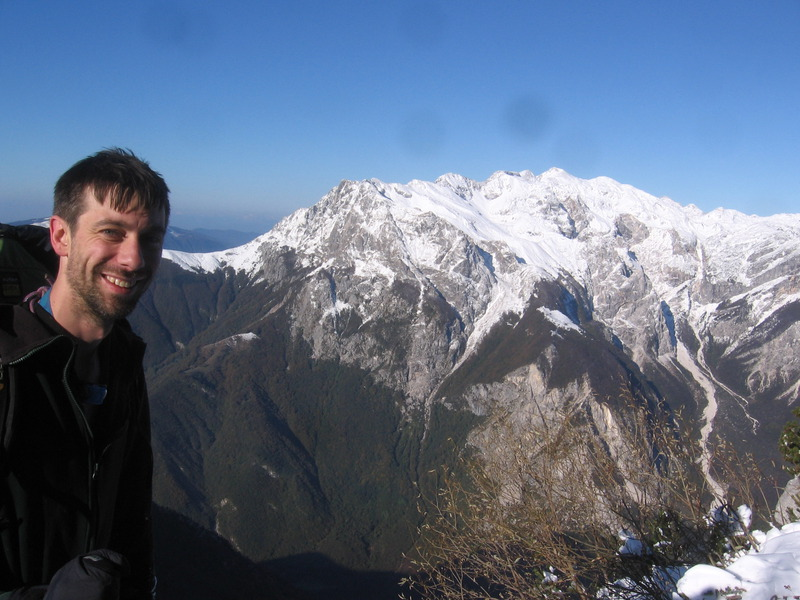
\includegraphics[width = \textwidth]{2011/super_action/Jarvist M Frost - Canon A520 - M2 Super Action - 2011-10-22-10.00.07-IMG_0185--orig.jpg}
\caption{The winter coat of \passage[mountain]{Krn}. \pic{Jarvist Frost}} \label{krn october}
\end{pagefigure}

Shortly after repacking our equipment, Izi arrives and we drive off to
\passage[town]{Tolminske Ravne}, the starting point for the trail to the \passage{Migovec
Plateau}. The trail is intimately familiar to anyone who has been on a
summer expedition, but at night, in the Fall and with a dusting of snow
it seemed strange. The crunch of the snow, boots on wet leaves, the
bubbles of light bobbing in the dark, give it an eerie quality. After an
hour or two we reach \passage{Kal}, the mountain hut of the Caving Section of the
Tolmin Alpine Club (JS-PDT). In the hut were \passage[town]{Tolmin} cavers Fratnik,
Samo, Zdenko and Maver (pronounced Mauw-er) and Grega from \passage[town]{Nova Gorica}.
Packs are dropped, boots swapped for slippers, sit beside the stove,
shake hands and greet everyone. Tradition dictates that the new guests
are offered fruit tea to rehydrate after the hike and a shot of liquor
for health. In this case the liquor is a particularly fine Jagermeister
made by Maver's grandmother. As soon as we are settled in, Izi and
Fratnik start preparing a large pot of pasta with tinned meat and tomato
sauce. A vast pot is soon standing in the middle of table and we all
tuck in. Rationally I know that we are eating from the pot to save
washing up, but a part of me believes that it is also a testimonial to
the spirit of sharing and the brotherhood of cavers. I am tempted to be
polite and only eat my share, taking spoons of pasta in turn. Tetley
turns to me, raises his eyebrows and says:

\begin{marginfigure}
\checkoddpage \ifoddpage \forcerectofloat \else \forceversofloat \fi
\centering
 \frame{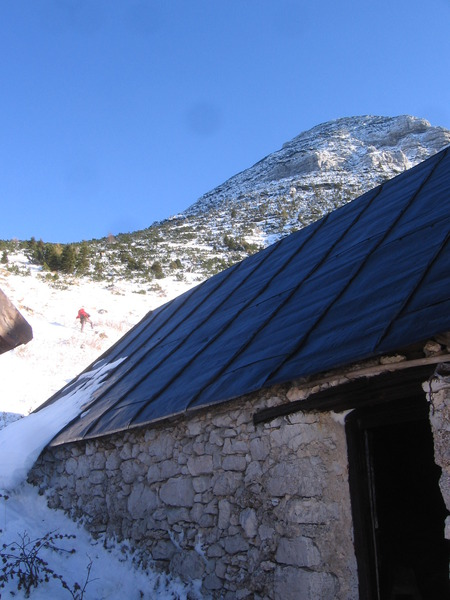
\includegraphics[width=\linewidth]{2011/super_action/Jarvist M Frost - Canon A520 - M2 Super Action - 2011-10-22-09.20.20-IMG_0184--orig.jpg}} 
 \caption{The face of \passage[mountain]{Migovec} overlooking \passage{Planina Kal}. \pic{Jarvist Frost}}
 \label{mig kal}
\end{marginfigure}

\begin{quote} Don't eat because you are hungry, eat because you want to get out of the cave tomorrow. \end{quote}

I follow his advice and proceed to gorge myself.

Soon more people start arriving: first the \passage[town]{Čadrg} people: Erik with
Karin and Tja\v{s}a, then Dejan and Bozo with two cavers from \passage[town]{Ljubljana}
Miha and Mojca (pronounced Moi-tz-a). More pasta is cooked, boxes of
wine appear, spirits are high, here is the creme de la creme of
cavers, Destiny weighs heavily on our shoulders, tomorrow the Connection
will be found. I notice that Fratnik has stopped drinking wine and
swapped to tea and take his lead ``I do not want to be completely
hungover tomorrow''. At some point we leave the hut to test out Bozo's
new petrol drill. It is huge ``how is he going to lug it through the
cave I wonder?'' Soon enough I fold for bed, full of dreams of the glory
that lies ahead.

The next day we wake up, have a summary breakfast of bread and pig fat
and pack up. In the meanwhile animated discussions in Slovenian are
determining the Plan for the day. Izi, Fratnik, Bozo, Dejan, Miha,
Mojca, Jarv and I will go to \passage{M2}, the rest will visit \passage{Primadona}.
Jarv and I have brought surveying equipment and our primary goal will be
to measure the finds from the past few years. The rest of the team will
travel to the bottom of the cave and continue the efforts to widen the
terminal rift. The rest of the \passage{M2} team has packed and gone. Bozo
is carrying the most terrifyingly large backpack I have ever seen. At
the last minute \bignote{Jarv and I realise we have not brought any food for
caving} and start scouring the hut looking for food. We managed to
scavenge 6 Frutabellas (yoghurt-fruit bars), a 200 g piece of bread and
a small (100 g) tin of tuna. In our minds we expect the surveying will
not take that long. Tetley also accompanies us up to the cave entrance.
Again walking up to \passage[mountain]{Mig} in the snow is a strange mix of familiar and
new. The usual path zig zags across the dwarf pine, but in the snow it
is possible to simply go straight up through or rather on top of the
vegetation. From the ridge of the mountain we can finally admire the
Plateau, it's covered in snow and a few hundred meters ahead of us is
the rest of the team. We walk on, passing the rock arch that we cook, eat
and live under during the summer. It is covered in a deep layer of snow,
but still is a familiar and loved place. Reaching \passage{M2}, we change
into our caving gear, bid farewell to Tetley and start caving. It is
11.30 a.m. when we start caving, we had set off from \passage{Kal} (the mountain
hut) two hours earlier.

\begin{marginfigure}
\checkoddpage \ifoddpage \forcerectofloat \else \forceversofloat \fi
\centering
 \frame{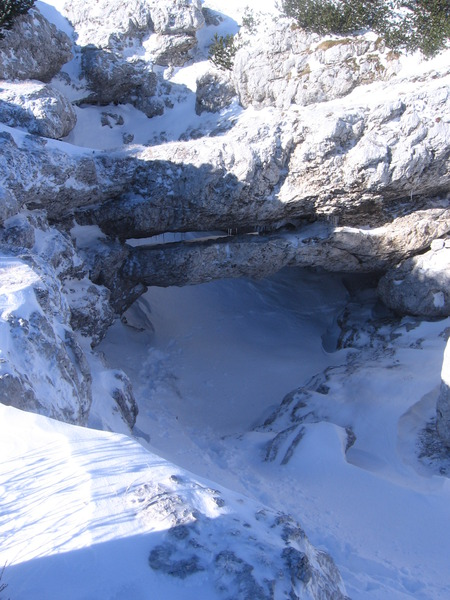
\includegraphics[width=\linewidth]{2011/super_action/Jarvist M Frost - Canon A520 - M2 Super Action - 2011-10-22-10.53.14-IMG_0199--orig.jpg}} 
 \caption{The \passage{bivi}, blanketed in snow. \pic{Jarvist Frost}}
 \label{snowy bivi}
\end{marginfigure}

\begin{pagefigure}
\checkoddpage \ifoddpage \forcerectofloat \else \forceversofloat \fi
   \centering
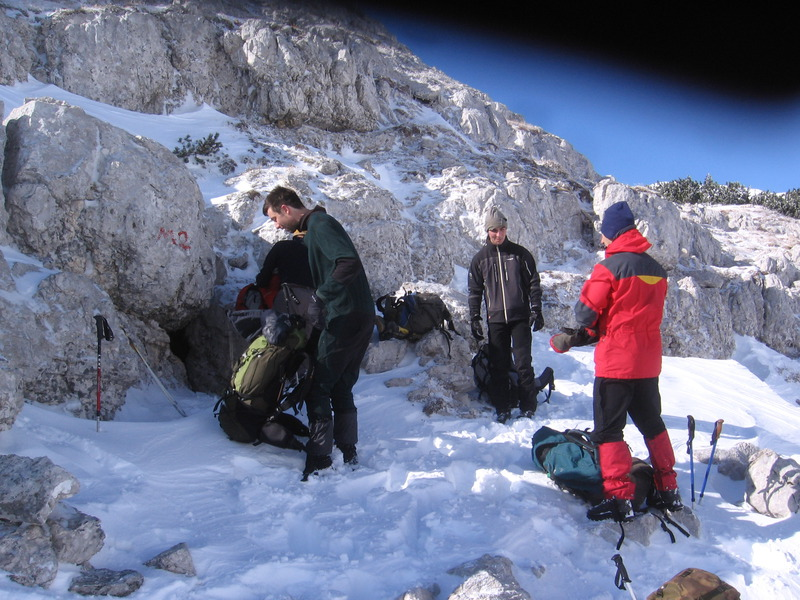
\includegraphics[width = \textwidth]{2011/super_action/Jarvist M Frost - Canon A520 - M2 Super Action - 2011-10-22-11.04.54-IMG_0202--orig.jpg}
\caption{Changing outside the entrance of \passage{M2}. \pic{Jarvist Frost}} \label{M2 october}
\end{pagefigure}

The entrance series of the cave has only two small pitches, the second
of which is permanently rigged with an aluminium ladder. The cave is a
long rift, constricted in a handful of places and certainly awkward if
carrying heavy tackle. After half an hour we reach the main pitch series
in the cave. First of all is \passage{Kletnik's shower}, this pitch is a long hang
in the drizzle. During a storm it can be very wet indeed, as Gergely and
Paul discovered in 2008\sidenote{see page XX from 2008}. After the shower, two more small pitches, some
more rift passage and we reach \passage{Silos}: a 100 m shaft discovered by the
Tolmin cavers in the '70s. Fratnik replaces one of the bolts and we all
pile on in. It is a truly awesome shaft, I have not been caving in a few
months and admit that I get in a bit of a bind on one of the rebelays,
the hand jammer has to come out of the bag  I hope none has noticed.
Later on Izi tells us that he has spied Fratnik using his cow's tails -- uncharacteristically cautious!

At the bottom of \passage{Silos} more rift and
a selection of short pitches leads to the '70s bottom of the cave. Again
there are quite a few section that could do with a little work with
hammer and chisel, but nothing is too horrendous. We pass the site of
the '70s camp. Some graffiti times the visit by the Tolmin cavers to
22-10-1977. \bignote{Exactly 34 years ago some of the people I am caving with
today were here}. We reach the limit of the survey and stop for lunch. It
is approximately 1.30 pm or so. Getting to the bottom of the cave has
taken 2 hours and I feel in great spirits, not cold, not sweaty, looking
forward to a tuna sandwich, a few hours of survey and out by sunset. We
share out the bread and eat our tuna. After the Slovenian cavers are
off, we sit in the Bothy bag that Jarv brought and have a little rest.
Neither of us has taken any tea or coffee this morning, so we eat a Pro
Plus to perk us up a little.

Soon Jarv and I start ascending the climb that Tim and Fratnik explored
in '09 and start surveying, Jarv takes book and instruments while I
operate the laser disto. A short climb and some meander leads to the
pushing front: a silted up rift. I poke my head in and feel
uncomfortable in the confined space. In my most reassuring voice I tell
Jarv: This is just the passage for you Jarv! You might want to take
your harness off. I then sit back and wait till Jarv wriggles his way
into a small chamber along the rift. He widens the passage a little by
removing some of the silt with the entrenching tool we found on site. We
both get a good feeling from this section. It drafts strongly and looks
exactly like the passage around \passage{Kill'em All}. We have to think of a name
for the passage. Impressed by Tim's effort in free climbing this, we
settle on \passage{Wizard of Oz}.


\begin{marginfigure}
\checkoddpage \ifoddpage \forcerectofloat \else \forceversofloat \fi
\centering
 \frame{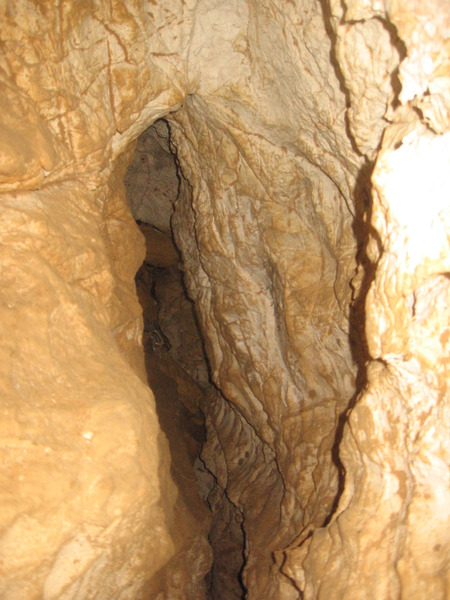
\includegraphics[width=\linewidth]{2011/super_action/Jarvist M Frost - Canon A520 - M2 Super Action - 2011-10-22-19.00.00-IMG_0212--orig.jpg}} 
 \caption{James wriggles into position in the rift in order to continue surveying in \passage{M2}. \pic{Jarvist Frost}} \label{M2 survey 1}
\end{marginfigure}

We return to the chamber where we had lunch and keep surveying down the
main passage. The rift has been widened, but surveying it still quite a
nuisance. We need to think of a new name, since the passage has been
widened so successfully with chocolate, we settle for \passage{Kinder
Surprise}.

\begin{figure}
\checkoddpage \ifoddpage \forcerectofloat \else \forceversofloat \fi
   \centering
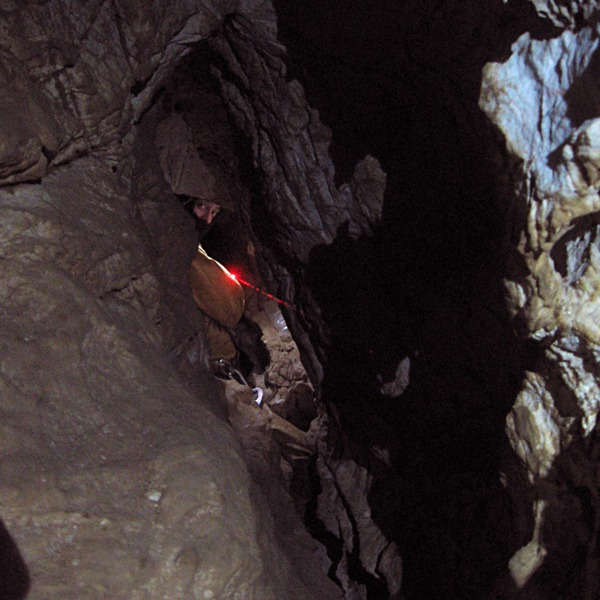
\includegraphics[width = \textwidth]{2011/super_action/Jarvist M Frost - Canon A520 - M2 Super Action - 2011-10-22-19.01.40-IMG_0215_square_crop_balanced--orig.jpg}
\caption{Looking back, surveying along the rift. \pic{Jarvist Frost}} \label{M2 survey 2}
\end{figure}

Eventually we reach the head of the large pitch that was discovered last
year. Here we meet the rest of the team, who are on the way out. The
pitch head is reached by climbing over a blind pot and I am sitting on
the edge of this pot, tied into the natural that forms the backup for
the pitch. First out is Bozo. I help him with his tackle sack and my arm
is almost wrenched out of its socket by the weight of it: petrol drills
are really heavy. Bozo seems a little downcast, apparently the efforts
to widen the rift at the pushing front have not been successful. It must
be depressing to have to carry the equipment out if it has not been
useful! After Bozo comes Fratnik and Izi. Eventually Jarv and I descend
the pitch, pass the last meander and reach the terminal chamber. There
is not much of a draft here, but you can definitely hear an echo. We can
see the marks from the drill. We settle on \passage{Echo Rift} as a good
name for this section of cave\sidenote{including the pitch} and start surveying back up the pitch.
Eventually our survey reconnects with the end of \passage{Kinder Surprise} and we
have finished our task. It is now more or less midnight. We have been
surveying for nine hours and it is time to get out. We have eaten all
our Frutabella bars and are now ravenously hungry.

The exit from the cave was honestly quite miserable. We were both
extremely low on energy, and despite taking another Pro Plus, I felt
rather sluggish. I tried to conserve my energy as much as possible,
knowing that many squeeze-climbs and crawl-traverses were waiting for me
on the way out and that each of these would require explosive power. So
we caved out, step after step, prussick stroke after prussick stroke. I
stopped after most large pitches and most squeezes to gain my breath. \bignote{I
checked and rechecked my bag to see if a chocolate bar had sneaked in}
somehow. On top of \passage{Silos} I sat down and closed my eyes. I did not fall
into a deep sleep, but into a dream-like state, when I heard the noise
of Jarv coming up behind me I was jolted back into the cave. We are
pretty much out, I kept repeating to myself, and at least the
squeezes get easier as you go further out. At 4.30 a.m. we were back
into the entrance of \passage{M2}. Luckily the weather was fine, no wind
and good vis.

Jarv successfully (miraculously?) navigated us back to the hut. I simply
put one foot in front of the other and fell over quite regularly.
Finally at 6.30 am. we were in \passage{Kal}, our mission was over. A nice plate
of jota and some tea and to sleep. The hut was even more packed than the
day before, people were taking turns for sleeping! It was nice to have
some company for dinner and I think our hosts were impressed that we had
been on such a long trip.

Next day we got back to town and entered the data into the survey. We
had surveyed 245 m of cave and added just over 100 m to the depth of
\passage{M2}. We had walked for 4 hrs in the snow and caved for 17 ½
hours. We ate approximately 1500 calories and consumed several thousand
more. We moved at an average speed of 3 meters per minute. We learnt
always to bring extra food. And then some more. The silted rift at the
end of \passage{Wizard of Oz} is about 4 meters horizontally (+/- 30) from a
survey leg at the edge of \passage{Dark Tranquillity}. The passage is heading
straight for \passage{Captain Kangaroo}. The enduring question is: will it go?

\name{James Kirkpatrick}

\begin{survey}
\checkoddpage \ifoddpage \forcerectofloat \else \forceversofloat \fi
   \centering
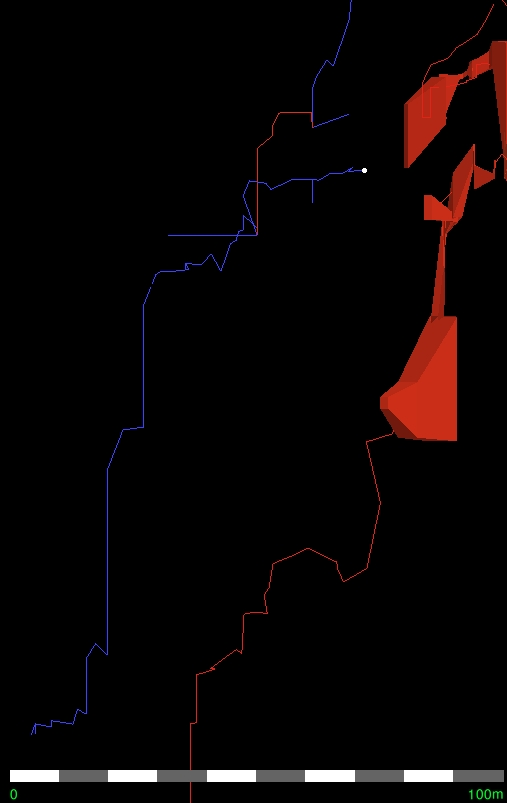
\includegraphics[width = \textwidth]{2011/super_action/m2-captk-2011--orig.jpg}
\caption[2011 Proximity of Wizard and Oz and Dark Tranquillity]{Extracted \textit{Aven} data showing the distance between \passage{Wizard of Oz} (highlighted with dot) in \passage{M2} (in blue/purple) and \passage{Dark Tranquillity} in \passage{Vrtnarija} (in red).} \label{M2CptK2011}
\end{survey}


\newpage



\begin{figure*}[t!]
\checkoddpage \ifoddpage \forcerectofloat \else \forceversofloat \fi
    \centering
        \frame{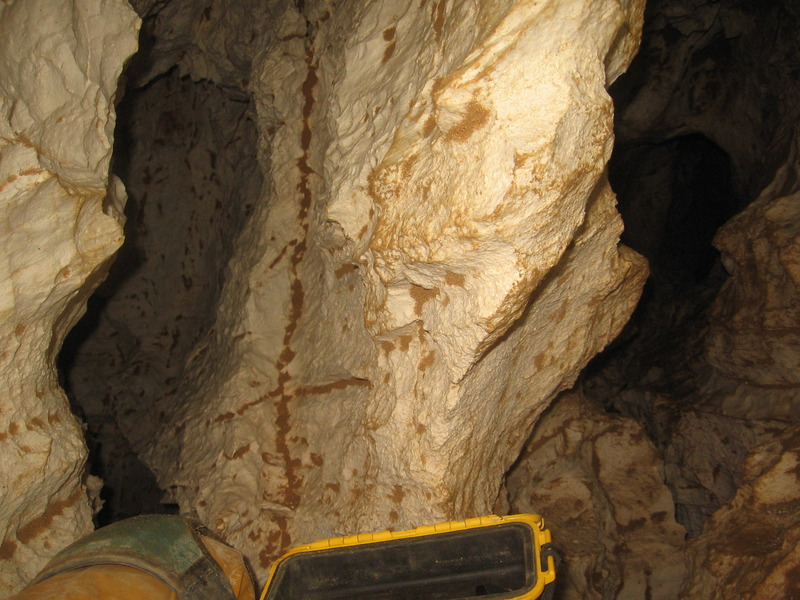
\includegraphics[width=\linewidth]{2011/super_action/Jarvist M Frost - Canon A520 - M2 Super Action - 2011-10-22-20.06.31-IMG_0217--orig.jpg}} 
 \caption{The tight corner at the Super Action's survey termination point in \passage{Kinder Surprise}, \passage{M2}. \pic{Jarvist Frost}} \label{tight rift termination M2}
\end{figure*}


\subsection{Additional Technical Notes}

On \passage{Kinder Surprise} we continued along the rift as we surveyed, missing the climb up into the rift that leads to the traverse over the pit to the large pitch\sidenote{\passage{Echo Rift} pitch}. The rift was increasingly tight and I stopped at a corner beyond which I'm certain from wear no one has passed. There is a small trickle of water audible, and I believe there is a small pitch beyond the short, tight, continuation of the rift. There is a PSS in the corner, in a crack in the rock. Though one might have imagined that these two bits of passage connect, the echo from the rift isn't really large enough and there wasn't any vocal contact with the Slovenians who must have been climbing the big pitch at this point. This might, therefore, still be a lead: Photograph taken from last PSS at end of tight rift on corner.
\name{Jarvist Frost}